カプセル化はエンドシステムでのみおこなわれ,ルータはRTPを送信するIPデータグラムか否かを判別できない.RTPは個別のパケットを個々のパケットのストリームに割り当てる.例えば,2人がビデオ会議をする際に,音声と映像について,それぞれ両方向に2つの流れ,計4つのストリームを割り当てる.しかしながらMPEG1やMPEG2は音声と映像を一つのストリームに割り当てるので両方向計2つのストリームで大丈夫である.RTPではセッションと呼ばれる参加者のグループが規定されており,参加者ごとのセッションの識別には、ネットワークアドレス、データを送信するポートの組、データを受信するポートの組が使用される.参加者は複数のセッションに同時に参加することも可能である.

\subsubsection{RTPヘッダフィールド}
RTPヘッダフィールドにはペイロードタイプ,シーケンス番号,タイムスタンプ,SSRC識別子が含まれている.ペイロードタイプは7bitで.音声,映像符号化の形式が含まれている.これにより受信側に通知する.続いて,シーケンス番号フィールドは16bit長でRTPが送られるたびにインクリメントを行い,受信者にパケットロスを通知し,パケットを回復する.86-89のシーケンス番号を送った時に87,88のパケットがロスしたと受信者に通知されたら,復旧させるように試みます.
タイムスタンプフィールドは32bit長で,受信側がネットワークで生成されたパケットの乱れを除去する,また,同期playoutを受信側に提供している.
SSRCはは32bitでRTPストリームのソースを識別するのに利用される.RTPセッションは区別されたSSRCを持っている.SSRCは送信側のIPアドレスではなく,新しいストリームが作られるたびにランダムに番号を割り振る.2つのストリームに同じ番号が割り振られるのは稀だが,起きた時は新しい番号を振り直す.

\subsection{SIP}
SIPはオープンで軽いプロトコルで,IPネットワークをもとに,発信者と着信者の間の通信でコールを確立する機構である.発信者が着信者に発信開始および終了の合図を行う.また発信者に受信者の現在のIPアドレスを通知している.また,コール管理の機構を提供している,コール中に新しいメディアストリームを加える,符号化を変更,コールに新しく参加者を加入させることとコール転送と,コール保留を行う.

\subsubsection{既知のIPアドレスとのコール確立}
SIPについて具体的に説明する.アリスがPCでボブのPCにコール設立をしたいとする.彼らのPCにはコールの送受信のSIPに基づいたソフトウェアが装備されているとする.まずアリスがボブに招待メッセージをUDPでウェルノウンポートである5060番ポートを送る.招待メッセージはボブの識別子,アリスの現在のIPアドレスの指示,アリスの受信フォーマット,アリスがRTPパケットを受信したいポート番号を含んでいる.受信後,ボブはSIPの応答メッセージを送信する.この応答メッセージは200 OKとボブのIPアドレスと受信フォーマットを含み,5060番ポートに送信される.ボブの応答後のアリスによるSIPのAckを送った後に,音声パケットをそれぞれ別のポートに送ることでアリスとボブが異なる符号化を利用することができる.これらの例から,SIPはout-of-bandプロトコルで,つまり,SIPメッセージは,メディアファイルを送受信するソケットと異なる場所を通じて送受信されることと,SIPメッセージはASCIIで可読性があり,HTTPメッセージに似ていること,メッセージに認証が必要であるため,UDP,TCP上で動くことがわかる.もし,ボブが符号化できない状況であったら200 OKの代わりに600 Not Acceptableを送信することで,アリスに招待メッセージを再送させる.

\subsubsection{SIPアドレス}
SIPアドレスとEmailアドレスは似ている.SIPアドレスを用いて,ボブにメッセージを送るときのようにIPアドレスにルーティングを行うことができる.このアドレスはWebページに貼り付けることができる.

\subsubsection{SIP招待メッセージ}
アリスがボブのSIPアドレスのみを知っており,IPアドレスを知らないときのアリスの招待メッセージに着目する.まずINVITE行にSIPのバージョンとSIPアドレスを表示している.Via行には通過する機器のIPアドレスを表示している.FromTo行はEmailと同じである.Call-ID行ではコールに識別子を割り振っている.Content-Type行ではSIPメッセージの内容を記述するのに利用されるフォーマットが記してあり,Content-Lengthには内容の長さ(byte)を表示している.その後,メッセージの内容が記述される.

\subsubsection{SIPプロキシ}
IPアドレスがDHCPで動的に割り当てられることが多く,ボブは複数の端末について,IPアドレスを所持しているため,アリスのSIP機器がボブのIPアドレスを知っているという仮定は非現実的である.アリスがボブのE-mailアドレスだけ知っていると仮定する.このアドレスを元に,ボブが利用しているデバイスのIPアドレスを特定するためにメッセージをSIPプロキシに送信する.その後プロキシはボブのE-mailアドレスで利用している機器のIPアドレスを含むSIPアドレスを返信する.プロキシからの返答は発信者によって異なる.

続いて,プロキシがボブの現在のIPアドレスを決定する際にSIPの機器の一つであるSIPレジストラについて述べる必要がある.全てのSIPユーザはレジストラを保持しており,ユーザ起動したSIPアプリケーションがSIP登録メッセージをレジストラに送信し、レジストラに現在のIPアドレスを通知する。ボブが新しいSIPアドレスに切り替えるたびに登録メッセージを送信し,同じデバイスに長期間止まっているときには,一定時間ごとに更新メッセージを送信するようにしている.多くの場合、SIPプロキシとSIPレジストラは同じホスト上で実行される.

例として,図\ref{fig:sip_registrar_and_proxy}を考える.送信側をjim@umass.edu, 受信側をkeith@upenn.eduとし,VoIP接続を行う.図\ref{fig:sip_registrar_and_proxy}において,まずジムが招待メッセージをSIPプロキシumass.eduに送信する(\raise0.2ex\hbox{\textcircled{\scriptsize{1}}}).その後,プロキシがupenn.eduでDNSルックアップ(DNSを用いて、ドメイン名やホスト名からIPアドレスを、あるいはその逆を調べること)を行い,メッセージをレジストラに送信する(\raise0.2ex\hbox{\textcircled{\scriptsize{2}}}).しかし受信側がもはやkeith@upenn.eduに登録されていないので,レジストラはリダイレクトを行い,keith@eurecom.frを試すよう指示する(\raise0.2ex\hbox{\textcircled{\scriptsize{3}}}).続いて,プロキシはSIPレジストラeurecom.frにINVITEメッセージを送信する(\raise0.2ex\hbox{\textcircled{\scriptsize{4}}}). eurecomレジストラはkeith@eurecom.frのIPアドレスを知っているため招待メッセージをホスト197.87.54.21に転送する(\raise0.2ex\hbox{\textcircled{\scriptsize{5}}}).その後応答を返信し
(\raise0.2ex\hbox{\textcircled{\scriptsize{6}}} $\sim$ \raise0.2ex\hbox{\textcircled{\scriptsize{8}}}),
メディアを送信する(\raise0.2ex\hbox{\textcircled{\scriptsize{9}}}).このようにして SIPは、一般に通話を開始および終了するためのプロトコルとしての役割を担っている.

\begin{figure}[tb]
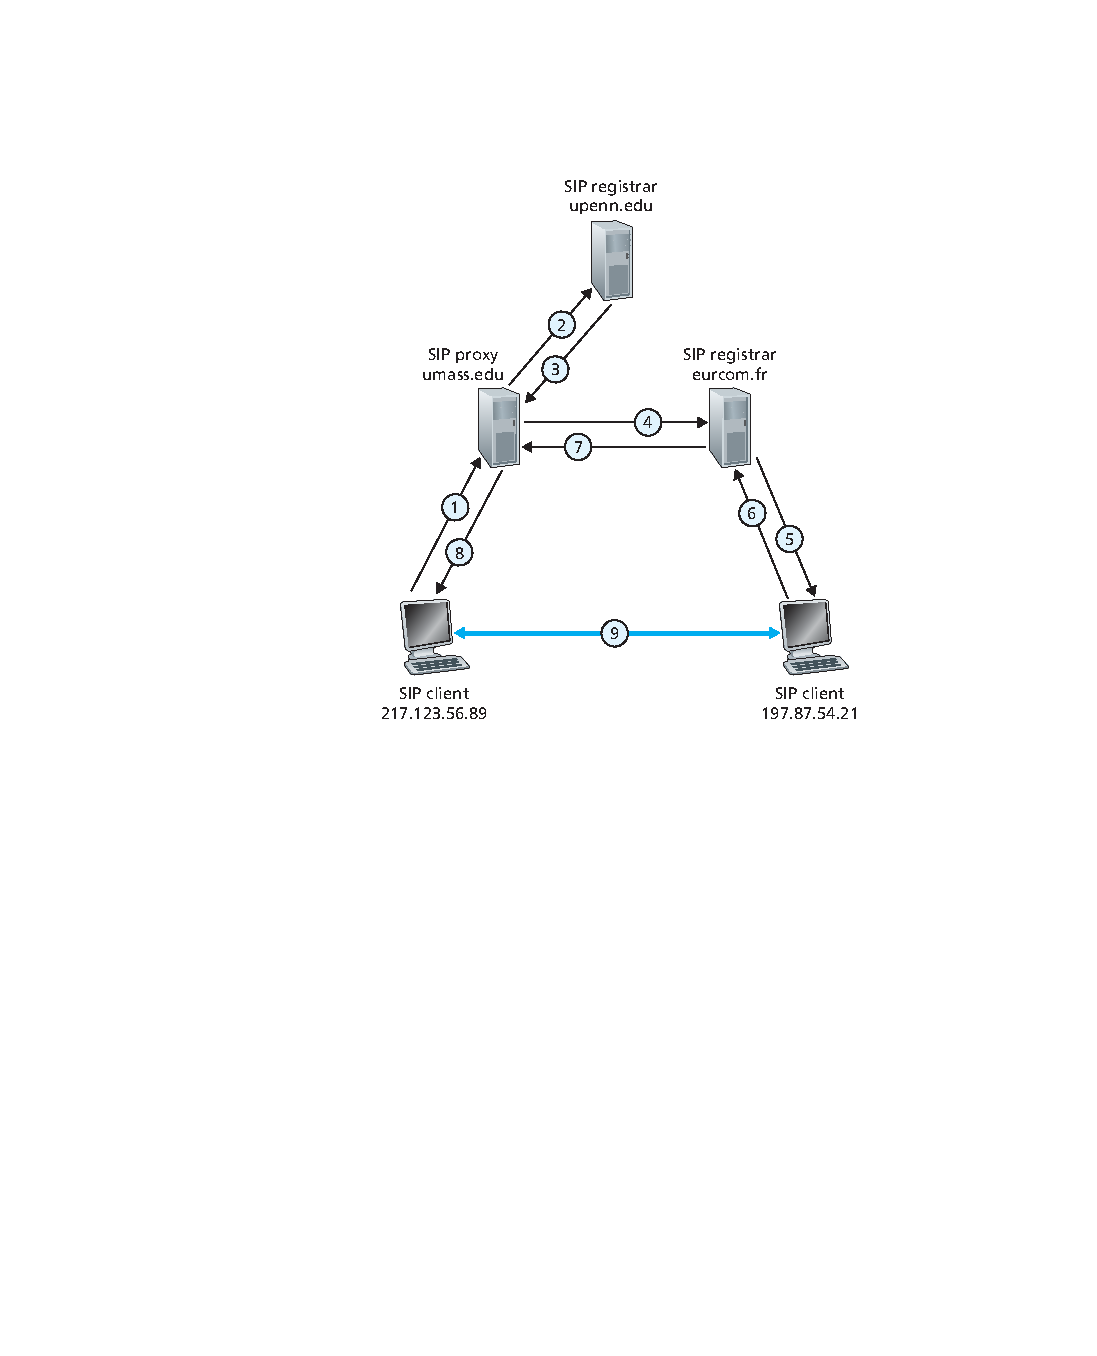
\includegraphics[width=10cm,pagebox=cropbox,clip]{sip_registrar_and_proxy.pdf}
 \caption{SIPプロキシとレジストラ}
 \label{fig:sip_registrar_and_proxy}
\end{figure}

\section{マルチメディアのためのネットワーク}
ここまではアプリケーションレベルでマルチメディアを説明した.また,コンテンツ配信ネットワークと,P2Pオーバーレイネットワークについても学んだ.しかし,アプリケーションレベルだけでなくネットワークもマルチメディアの送受信を支援する機構を保持している.ただ,この機構は新しいのでまだ普及されていない.

\end{document}
